\chapter{麥克斯威方程、協變性與電磁波}

\lectureoverview{電場和磁場透過洛倫茲力作用於帶電物質，但物質也會產生並重新分布場。我們將探討電磁學中物質對場作用的這一面，說明麥克斯威方程具有洛倫茲協變性，推導其波動解，最後以能明確呈現局域守恆的形式重新納入電荷和電流。整堂課都採用\(c=1\)的單位制。}

\section{電磁學的另一面}

先從已經學過的部分開始。若一個電荷為\(q\)的粒子以速度\(\mathbf v\)穿越電場和磁場，所受的力為
\begin{equation}
\mathbf F=q\bigl(\mathbf E+\mathbf v\times\mathbf B\bigr).
\label{eq:lorentz-force-three}
\end{equation}
因子\(q\)不可或缺。中性粒子不會受到電磁力。即使粒子瞬間靜止，電場仍會產生作用；磁場的作用則取決於粒子的運動。

方程~\eqref{eq:lorentz-force-three}告訴我們給定的場如何作用於物質，卻沒有說明場是由什麼決定的。是什麼在某個物體周圍產生電場、在另一個物體周圍產生磁場，或在真空中產生傳播的波？回答這些問題的就是麥克斯威方程。

\begin{figure}[H]
\centering
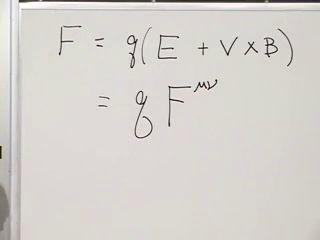
\includegraphics[width=0.62\textwidth]{lecture_58_figure_02.png}
\caption{三維向量形式的洛倫茲力，以及將其改寫為張量形式的開端。}
\lectureframe{00:05:49}
\end{figure}

力定律的相對論形式預示了接下來要用的記號：
\begin{equation}
f^\mu=qF^\mu{}_{\nu}u^\nu.
\label{eq:lorentz-force-four}
\end{equation}
其中，\(u^\nu\)是四速度，\(f^\mu\)是四力，而\(F^{\mu\nu}\)是由\(\mathbf E\)和\(\mathbf B\)組成的反對稱張量。黑板上先只寫出這個表示式的示意性開頭；與\(u^\nu\)縮並後，才會得到留下單一自由力指標所需的向量。

物質必須反過來作用於場，這有其物理理由。電磁波可以撞上電荷，使它加速，並將能量傳給它。如果場能影響電荷，而電荷卻永遠不能影響場，那麼場傳給電荷的能量就無從而來。作用與反作用還不足以說明全部，但能量守恆使這種相互耦合不可避免。

\section{變動的源會發出擾動}

點電荷會產生一個從其位置向外或向內指向的電場。導線中的電流--也就是帶電粒子的流動--則會產生環繞導線的磁場。這些熟悉的靜態圖像已呈現兩種不同的幾何形態：電通量由電荷向外發出，磁力線則環繞電流。

現在讓點電荷突然移動。在它的新位置附近，電場必須開始重新分布；但遠方的觀察者不可能立即得知它已移動。在訊號抵達之前，遠方的舊場仍維持原狀。近處與遠處之間有一道移動的前沿，場在此處發生變化。這道移動中的場變化就是電磁擾動。

若電荷來回振盪，連續的場變化便接踵而至，形成電磁波。這就是天線的基本作用：振盪電流向外發出場的擾動。將導線中的電流反向，也可用同樣的論證說明磁場的情形。\(\mathbf B\)的環流必須反向，但這個變化會向外傳播，不會同時出現在各處。

這個因果圖像為麥克斯威方程設定了兩個目標：描述電荷和電流如何作為場的源，並允許場的變化以不超過光速的速度傳播。第二個目標也可用來檢驗相對論。如果麥克斯威方程在每個慣性參考系中形式相同，且蘊含一個確定的波速，那麼每個慣性參考系都必須從中推得相同的速度。

\section{回顧相對論波動方程}

在討論向量場之前，先考慮標量場\(\phi(\mathbf x,t)\)，也就是時空中每一點都有一個數值的場。一個一階導數方程
\begin{equation}
\partial_\mu\phi=0
\end{equation}
表示所有時空方向的導數都為零。這樣的場會是常數，因此無法承載波。非平凡的相對論波動方程需要二階導數：
\begin{equation}
\partial_\mu\partial^\mu\phi=0.
\end{equation}
按照這裡採用的符號慣例，
\begin{equation}
\left(\partial_t^2-\partial_x^2-\partial_y^2-\partial_z^2\right)\phi=0,
\label{eq:scalar-wave-four}
\end{equation}
也可以更精簡地寫成
\begin{equation}
\left(\partial_t^2-\nabla^2\right)\phi=0.
\end{equation}
採用\(c=1\)，可使時間和距離使用相容的單位。恢復一般單位制時，二階時間導數前會出現\(1/c^2\)。

若波沿\(z\)軸傳播，場只依賴\(z\)和\(t\)，不依賴\(x\)或\(y\)。方程~\eqref{eq:scalar-wave-four}便化為
\begin{equation}
\left(\partial_t^2-\partial_z^2\right)\phi=0.
\label{eq:scalar-wave-one}
\end{equation}

\begin{figure}[H]
\centering
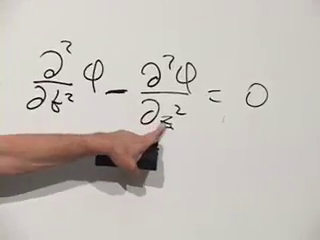
\includegraphics[width=0.56\textwidth]{lecture_58_figure_04.png}
\caption{作為電磁波模型的一維標量波動方程。}
\lectureframe{00:47:03}
\end{figure}

其一般行波解為
\begin{equation}
\phi(z,t)=f(z-t)+g(z+t).
\end{equation}
波形\(f(z-t)\)沿\(z\)增大的方向傳播，因為相位固定的點滿足\(z-t=\text{constant}\)。波形\(g(z+t)\)則朝相反方向傳播。兩個波形都不必是正弦波；只要形狀足夠平滑，就能在平移時維持原形。

不過，正弦波很方便使用：
\begin{equation}
\phi(z,t)=A\cos\!\bigl(k(z-t)\bigr).
\end{equation}
波數\(k\)決定波長，
\begin{equation}
\lambda=\frac{2\pi}{k}.
\end{equation}
\(k\)較大時，空間振盪較快、波長較短；\(k\)較小時，波長較長。這些波形很快就會成為\(\mathbf E\)和\(\mathbf B\)的分量。

\section{麥克斯威方程所需的向量微積分}

麥克斯威方程以點積、叉積、散度和旋度表示。值得先重新整理一次這些記號，因為後續的分量計算會用到這些運算形式。

對一般三維向量\(\mathbf a\)和\(\mathbf b\)而言，點積是純量：
\begin{equation}
\mathbf a\cdot\mathbf b
=a_xb_x+a_yb_y+a_zb_z.
\end{equation}
叉積則是另一個向量：
\begin{align}
(\mathbf a\times\mathbf b)_x&=a_yb_z-a_zb_y,\\
(\mathbf a\times\mathbf b)_y&=a_zb_x-a_xb_z,\\
(\mathbf a\times\mathbf b)_z&=a_xb_y-a_yb_x.
\end{align}
其餘分量可依循環順序\(x\to y\to z\to x\)得到。

引入微分算子
\begin{equation}
\boldsymbol\nabla=
\left(\partial_x,\partial_y,\partial_z\right).
\end{equation}
它的分量是算子而非一般數值，但仍可依照點積和叉積的運算形式計算。對向量場\(\mathbf A\)而言，
\begin{equation}
\boldsymbol\nabla\cdot\mathbf A
=\partial_xA_x+\partial_yA_y+\partial_zA_z
\label{eq:divergence}
\end{equation}
是散度；
\begin{align}
(\boldsymbol\nabla\times\mathbf A)_x
 &=\partial_yA_z-\partial_zA_y,\\
(\boldsymbol\nabla\times\mathbf A)_y
 &=\partial_zA_x-\partial_xA_z,\\
(\boldsymbol\nabla\times\mathbf A)_z
 &=\partial_xA_y-\partial_yA_x
\label{eq:curl}
\end{align}
則是旋度的各分量。

幾何圖像和公式同樣重要。向量場看起來由某處向外流出時，該處的散度為正；場呈環流狀時，則有旋度。點電荷的徑向電場可說明散度，載流導線周圍環繞的磁場則可說明旋度。空間中均勻的向量場兩者皆無。

\section{真空中的麥克斯威方程}

沒有電荷和電流時，麥克斯威方程為
\begin{align}
\boldsymbol\nabla\times\mathbf E&=-\partial_t\mathbf B,
\label{eq:faraday-vac}\\
\boldsymbol\nabla\cdot\mathbf B&=0,
\label{eq:gauss-b-vac}\\
\boldsymbol\nabla\times\mathbf B&=\partial_t\mathbf E,
\label{eq:ampere-vac}\\
\boldsymbol\nabla\cdot\mathbf E&=0.
\label{eq:gauss-e-vac}
\end{align}
兩個旋度方程幾乎可以互換\(\mathbf E\)與\(\mathbf B\)，但關鍵的負號使兩者有所不同。兩個散度方程則表示，在所考慮的真空區域內，兩個場都沒有源。即使重新納入電荷源，磁場的散度仍為零；一般電磁學不包含磁荷。

\begin{figure}[H]
\centering
\includegraphics[width=0.76\textwidth]{lecture_58_figure_06.png}
\caption{四個真空中的麥克斯威方程，排列方式呈現電場與磁場之間近似的對稱性。}
\lectureframe{00:27:30}
\end{figure}

最後，電荷密度\(\rho\)會取代方程~\eqref{eq:gauss-e-vac}右側的零，而電流密度\(\mathbf J\)會出現在方程~\eqref{eq:ampere-vac}中。這些項目暫且先不納入。無源方程的形式較簡潔，能清楚呈現變換結構和波的形成機制。

它們也讓愛因斯坦的難題更加尖銳。若以伽利略變換描述一位隨波移動的觀察者，他會預期速度相減，測得較小的波速。然而，若麥克斯威方程在每個慣性參考系中都成立，每位觀察者就都會推得相同的單位波速。解決之道不是在不同參考系中改變波動方程，而是使用洛倫茲變換，並以變換律已知的物件來表示麥克斯威方程。

\section{電場與磁場組成同一個張量}

電場和磁場組合成反對稱的場張量
\begin{equation}
F^{\mu\nu}=
\begin{pmatrix}
0   & -E_x & -E_y & -E_z\\
E_x & 0    & -B_z & B_y\\
E_y & B_z  & 0    & -B_x\\
E_z & -B_y & B_x  & 0
\end{pmatrix},
\label{eq:l0203-field-tensor}
\end{equation}
矩陣的列與行依\(t,x,y,z\)排列。反對稱性
\begin{equation}
F^{\mu\nu}=-F^{\nu\mu},
\end{equation}
使對角元素必為零，也決定了矩陣下半部的元素由上半部給出。時間與空間方向交錯的元素包含\(\mathbf E\)；純空間方向的元素則包含\(\mathbf B\)。

\begin{figure}[H]
\centering
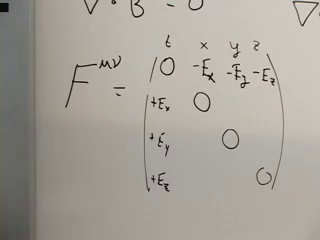
\includegraphics[width=0.58\textwidth]{lecture_58_figure_03.png}
\caption{完整的電磁場張量，包含電場與磁場的元素。}
\lectureframe{00:32:05}
\end{figure}

\(F^{\mu\nu}\)的重要性不只在於能將六個場分量收納在同一個矩陣中。在洛倫茲變換下，它依照二階張量的變換律變換。因此，不同觀察者測得的電場和磁場會恰當地混合，使整個張量能一致地變換。

還有另一個反對稱張量，稱為對偶場張量\(\widetilde F^{\mu\nu}\)。依照目前採用的慣例，從方程~\eqref{eq:l0203-field-tensor}出發，以如下替換
\begin{equation}
\mathbf E\longmapsto-\mathbf B,
\qquad
\mathbf B\longmapsto\mathbf E.
\label{eq:dual-replacement}
\end{equation}
便可得到對偶張量：
\begin{equation}
\widetilde F^{\mu\nu}=
\begin{pmatrix}
0    & B_x  & B_y  & B_z\\
-B_x & 0    & -E_z & E_y\\
-B_y & E_z  & 0    & -E_x\\
-B_z & -E_y & E_x  & 0
\end{pmatrix}.
\label{eq:dual-tensor}
\end{equation}
方程~\eqref{eq:dual-replacement}中的符號至關重要。講課時先口頭交換電場與磁場，隨即發現符號不符，於是先修正符號，再完成矩陣。

\begin{figure}[H]
\centering
\includegraphics[width=0.58\textwidth]{lecture_58_figure_07.png}
\caption{以必要的符號交換電場與磁場元素，組成對偶張量。}
\lectureframe{00:35:45}
\end{figure}

\section{協變形式的真空方程}

每個麥克斯威方程都含有一個導數。從二階張量出發，將一個指標與導數縮並後，會留下一個自由指標，因此自然的協變形式候選式為
\begin{align}
\partial_\mu F^{\mu\nu}&=0,
\label{eq:maxwell-covariant-vac}\\
\partial_\mu\widetilde F^{\mu\nu}&=0.
\label{eq:maxwell-dual-vac}
\end{align}
固定\(\nu\)後，方程~\eqref{eq:maxwell-covariant-vac}就是一條方程。由於\(\nu\)可以取\(t,x,y,z\)，這個式子涵蓋四條純量方程。方程~\eqref{eq:maxwell-dual-vac}則涵蓋另外四條。這正好對應原先列出的兩個向量旋度方程和兩個純量散度方程。

緊湊的記號必須能重現熟悉的方程才有用。取\(\nu=z\)：
\begin{align}
\partial_\mu F^{\mu z}
&=\partial_tF^{tz}
  +\partial_xF^{xz}
  +\partial_yF^{yz}
  +\partial_zF^{zz}\\
&=-\partial_tE_z+\partial_xB_y-\partial_yB_x\\
&=-\partial_tE_z+
  \bigl(\boldsymbol\nabla\times\mathbf B\bigr)_z.
\end{align}
項\(F^{zz}\)因反對稱性而消失。令結果等於零，就得到
\(z\)分量的方程：
\begin{equation}
\boldsymbol\nabla\times\mathbf B=\partial_t\mathbf E.
\end{equation}
\(x\)和\(y\)分量則可循環更換指標得到。

\begin{figure}[H]
\centering
\includegraphics[width=0.76\textwidth]{lecture_58_figure_08.png}
\caption{協變場方程的分量展開：對角張量元素為零，其餘項則還原出麥克斯威方程。}
\lectureframe{00:43:30}
\end{figure}

接著取時間分量：
\begin{align}
\partial_\mu F^{\mu t}
&=\partial_tF^{tt}
  +\partial_xF^{xt}
  +\partial_yF^{yt}
  +\partial_zF^{zt}\\
&=\partial_xE_x+\partial_yE_y+\partial_zE_z\\
&=\boldsymbol\nabla\cdot\mathbf E.
\end{align}
這便得到方程~\eqref{eq:gauss-e-vac}。對偶張量也可用同樣方式檢查，得到
\(\boldsymbol\nabla\cdot\mathbf B=0\)以及
\(\boldsymbol\nabla\times\mathbf E=-\partial_t\mathbf B\)。

現在已經推導出這些緊湊方程，而非僅僅猜測它們。自由指標的結構使它們成為四向量方程，因此洛倫茲變換會改變方程的分量，卻不改變其形式。這就是真空中的麥克斯威方程在每個慣性參考系中形式相同的確切意義。

\section{從一階方程推得波動方程}

麥克斯威方程只含一階導數，而波動方程含有二階導數。這看似不一致，但麥克斯威理論耦合了兩個場，因此可以將\(\mathbf E\)和\(\mathbf B\)的一對一階方程合併，得到任一場各自滿足的二階方程。

將方程~\eqref{eq:ampere-vac}對時間微分：
\begin{equation}
\partial_t^2\mathbf E
=\boldsymbol\nabla\times\partial_t\mathbf B.
\end{equation}
法拉第定律給出\(\mathbf B\)的時間導數：
\begin{equation}
\partial_t\mathbf B=-\boldsymbol\nabla\times\mathbf E,
\end{equation}
因此
\begin{equation}
\partial_t^2\mathbf E
=-\boldsymbol\nabla\times
  \bigl(\boldsymbol\nabla\times\mathbf E\bigr).
\label{eq:double-curl}
\end{equation}

黑板上的推導逐一計算各分量，並未直接引用熟記的恆等式。以\(x\)分量為例：
\begin{align}
\bigl[\boldsymbol\nabla\times
(\boldsymbol\nabla\times\mathbf E)\bigr]_x
&=\partial_y(\boldsymbol\nabla\times\mathbf E)_z
 -\partial_z(\boldsymbol\nabla\times\mathbf E)_y\\
&=\partial_y(\partial_xE_y-\partial_yE_x)\\
&\quad-\partial_z(\partial_zE_x-\partial_xE_z)\\
&=\partial_x(\partial_yE_y+\partial_zE_z)
 -\partial_y^2E_x\\
&\quad-\partial_z^2E_x.
\end{align}
加上再減去\(\partial_x^2E_x\)，即可整理出散度：
\begin{align}
\bigl[\boldsymbol\nabla\times
(\boldsymbol\nabla\times\mathbf E)\bigr]_x
&=\partial_x(\boldsymbol\nabla\cdot\mathbf E)
 -\nabla^2E_x.
\label{eq:double-curl-x}
\end{align}
在真空中，\(\boldsymbol\nabla\cdot\mathbf E=0\)。合併方程~\eqref{eq:double-curl}與\eqref{eq:double-curl-x}，得到
\begin{equation}
\left(\partial_t^2-\nabla^2\right)E_x=0.
\label{eq:ex-wave}
\end{equation}

\begin{figure}[H]
\centering
\includegraphics[width=0.72\textwidth]{lecture_58_figure_09.png}
\caption{逐分量計算後，得到\(E_x\)的波動方程。}
\lectureframe{00:57:10}
\end{figure}

同樣的計算也適用於\(E_y\)和\(E_z\)，以類似方式消去另一個場後可得
\begin{equation}
\left(\partial_t^2-\nabla^2\right)\mathbf B=0.
\end{equation}
因此，電場和磁場都能以波的形式在真空中傳播。採用這裡的單位制時，波速為一；恢復一般單位後，波速就是\(c\)。

\section{平面波與偏振}

考慮一個沿\(z\)正方向傳播的簡單波：
\begin{equation}
\mathbf E(z,t)
=\widehat{\mathbf x}\,E_0
  \cos\!\bigl(k(z-t)\bigr).
\label{eq:plane-e}
\end{equation}
波形沿\(z\)方向平移而不改變形狀。由於電場沿\(x\)軸，這個波在\(x\)方向上呈線偏振。我們選擇\(E_y=0\)只是為了簡化例子；也可以加入第二種橫向偏振。

縱向分量則不能任意變化。由於波只依賴\(z\)和\(t\)，
\begin{equation}
\boldsymbol\nabla\cdot\mathbf E
=\partial_zE_z=0.
\end{equation}
所以\(E_z\)可以是常數，卻不能包含隨波變化的部分。均勻背景場可以獨立地疊加或移除，但它不屬於傳播中的輻射。波本身是橫向的：
\begin{equation}
\mathbf E_{\mathrm{wave}}\cdot\widehat{\mathbf z}=0.
\end{equation}

法拉第定律決定了磁場。對於方程~\eqref{eq:plane-e}，\(\boldsymbol\nabla\times\mathbf E\)只有\(y\)分量不為零：
\begin{equation}
(\boldsymbol\nabla\times\mathbf E)_y=\partial_zE_x.
\end{equation}
因此\(\partial_t\mathbf B\)沿\(y\)方向；一個符合條件的選擇是
\begin{equation}
\mathbf B(z,t)
=\widehat{\mathbf y}\,E_0
  \cos\!\bigl(k(z-t)\bigr).
\label{eq:plane-b}
\end{equation}
在這個單位制下，電場和磁場的振幅相等。兩者的方向關係為
\begin{equation}
\mathbf E\perp\mathbf B,
\qquad
\mathbf E\perp\widehat{\mathbf z},
\qquad
\mathbf B\perp\widehat{\mathbf z},
\qquad
\mathbf E\times\mathbf B\parallel\widehat{\mathbf z}.
\end{equation}

\begin{figure}[H]
\centering
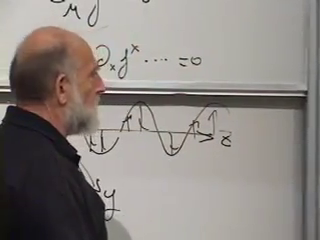
\includegraphics[width=0.70\textwidth]{lecture_58_figure_05.png}
\caption{完整的黑板示意圖呈現橫電磁波：電場和磁場的振盪彼此垂直，且都垂直於傳播方向。}
\lectureframe{01:05:25}
\end{figure}

\begin{figure}[H]
\centering
\scalebox{0.90}{%
\begin{tikzpicture}[x=1cm,y=1cm,>=Latex]
  \draw[->,thick] (0,0) -- (8.2,0) node[right] {$z$};
  \draw[->,thick] (0,-1.6) -- (0,1.7) node[above] {$x$};
  \draw[->,thick] (0,0) -- (-1.15,-0.8) node[below left] {$y$};
  \draw[blue!70!black,thick,domain=0:7.5,samples=120]
    plot (\x,{0.95*sin(90*\x)});
  \foreach \z/\s in {0.8/1,2.8/-1,4.8/1,6.8/-1}{
    \draw[->,green!45!black,thick]
      (\z,0) -- ++({-0.55*\s},{-0.38*\s});
  }
  \node[blue!70!black] at (6.9,1.25) {$\mathbf E$};
  \node[green!45!black] at (5.2,-1.05) {$\mathbf B$};
  \draw[->,very thick] (6.2,1.55) -- (7.7,1.55)
    node[midway,above] {propagation};
\end{tikzpicture}
}
\caption{場\(\mathbf E\)和\(\mathbf B\)彼此垂直，且都垂直於傳播方向。}
\end{figure}

這就是光以及所有真空中電磁輻射的特性。由於導出此波的方程具有洛倫茲協變性，另一位慣性觀察者也會描述一個以\(c\)傳播、具有橫向電場和磁場的電磁波。

\section{電荷密度與電流密度}

現在重新納入先前暫時擱置的源。當許多帶電粒子分布在一個區域內時，可將其粗粒化，並以連續的電荷密度描述：
\begin{equation}
\rho(\mathbf x,t)=\frac{dQ}{dV}.
\end{equation}
這種近似就像將水視為連續流體，儘管水是由分子組成。正電荷和負電荷的貢獻符號相反，因此\(\rho\)代表每單位體積的淨電荷。

選定區域\(V\)內的電荷為
\begin{equation}
Q_V(t)=\int_V\rho(\mathbf x,t)\,dV.
\label{eq:charge-volume}
\end{equation}
電荷密度可以隨位置和時間變化。一團電荷移離某點時，該處的局域密度便會改變。但電荷密度不能任意變化，因為電荷守恆。

只要求總量守恆還不夠。這會容許電荷在同一瞬間從地球消失、又在火星出現，只要總量不變即可。更強的局域守恆敘述是：電荷只能經由中間空間中的流動，從一處離開並抵達另一處。

為描述這種流動，取一個無窮小的有向面積元素
\begin{equation}
d\boldsymbol\sigma=\widehat{\mathbf n}\,d\sigma.
\end{equation}
其大小為面積，方向則垂直於表面。電流密度\(\mathbf J\)的定義是：單位時間內穿過此面積元素的電荷量為
\begin{equation}
\frac{dQ}{dt}=\mathbf J\cdot d\boldsymbol\sigma.
\label{eq:current-flux-element}
\end{equation}
\(\mathbf J\)的大小表示單位面積、單位時間內通過的電荷量，方向則與正電荷流動方向一致。

\begin{figure}[H]
\centering
\includegraphics[width=0.64\textwidth]{lecture_58_figure_10.png}
\caption{有向面積元素與通量因子\(d\boldsymbol\sigma\cdot\mathbf J\)。}
\lectureframe{01:18:15}
\end{figure}

點積會選出垂直於表面的分量。沿表面切向流動的電流不會穿過表面的任一側，因此通量為零。若電流平行於法線，在電流大小固定時，通量最大。導線中的電流只是其中一種情況；\(\mathbf J\)也可以描述電荷流經薄片，或在整個三維空間中流動。

\section{局域守恆與連續方程}

固定空間中的區域\(V\)，並使其封閉邊界\(\partial V\)上的每個面積元素都朝外取向。若有淨電流向外流出，區域內的電荷量便會減少：
\begin{equation}
\frac{dQ_V}{dt}
=-\oint_{\partial V}\mathbf J\cdot d\boldsymbol\sigma.
\label{eq:integral-conservation}
\end{equation}
這個負號反映的是物理意義，而非記號慣例：向外的正通量會帶走區域內的正電荷。利用方程~\eqref{eq:charge-volume}，可得
\begin{equation}
\int_V\partial_t\rho\,dV
=-\oint_{\partial V}\mathbf J\cdot d\boldsymbol\sigma.
\label{eq:integral-continuity-one}
\end{equation}

\begin{figure}[H]
\centering
\includegraphics[width=0.72\textwidth]{lecture_58_figure_11.png}
\caption{將表面通量轉寫為體積積分後，固定區域的守恆定律。}
\lectureframe{01:29:00}
\end{figure}

高斯定理，也稱為散度定理，將穿過封閉曲面的通量與曲面內部的散度連結起來：
\begin{equation}
\oint_{\partial V}\mathbf A\cdot d\boldsymbol\sigma
=\int_V\boldsymbol\nabla\cdot\mathbf A\,dV.
\label{eq:divergence-theorem}
\end{equation}
可以想像容器內有看不見的管道，在內部各處注入水。散度衡量水從管道出口流出的局域速率；曲面積分則衡量離開容器的水量總和。容器內部產生的向外流動，最終都必須穿過邊界。

將方程~\eqref{eq:divergence-theorem}應用於\(\mathbf J\)，得到
\begin{equation}
\int_V
\left(\partial_t\rho+\boldsymbol\nabla\cdot\mathbf J\right)dV=0.
\end{equation}
此關係對每一個可能的區域\(V\)都成立。因此，被積函數必須在每一點都為零：
\begin{equation}
\boxed{\partial_t\rho+\boldsymbol\nabla\cdot\mathbf J=0.}
\label{eq:continuity-three}
\end{equation}

\begin{figure}[H]
\centering
\includegraphics[width=0.72\textwidth]{lecture_58_figure_12.png}
\caption{以分量形式表示的局域連續方程。}
\lectureframe{01:29:50}
\end{figure}

方程~\eqref{eq:continuity-three}正是局域守恆所要求的條件。如果某點或某個小區域內的電荷密度減少，電流就必須從該處向外發散；如果電流向內匯聚，電荷密度便會增加。

電荷密度與電流自然地組成四電流
\begin{equation}
J^\mu=(\rho,J_x,J_y,J_z)
\label{eq:four-current}
\end{equation}
單位制採用\(c=1\)時，連續方程可寫成洛倫茲純量方程
\begin{equation}
\partial_\mu J^\mu=0.
\label{eq:continuity-four}
\end{equation}
相對論性分布的流量應像單一粒子的四速度一樣，依四向量的變換律變換。方程~\eqref{eq:continuity-four}確保局域電荷守恆在每個慣性參考系中都成立。

\section{有源麥克斯威方程}

重新納入電荷和電流後，得到
\begin{align}
\boldsymbol\nabla\cdot\mathbf E&=\rho,
\label{eq:gauss-e-source}\\
\boldsymbol\nabla\cdot\mathbf B&=0,\\
\boldsymbol\nabla\times\mathbf E&=-\partial_t\mathbf B,\\
\boldsymbol\nabla\times\mathbf B&=\partial_t\mathbf E+\mathbf J.
\label{eq:ampere-source}
\end{align}
涉及電場源的方程可合併為
\begin{equation}
\boxed{\partial_\mu F^{\mu\nu}=J^\nu,}
\label{eq:maxwell-source-covariant}
\end{equation}
而磁場的無源方程仍為
\begin{equation}
\boxed{\partial_\mu\widetilde F^{\mu\nu}=0.}
\label{eq:maxwell-dual-source}
\end{equation}

\begin{figure}[H]
\centering
\includegraphics[width=0.78\textwidth]{lecture_58_figure_13.png}
\caption{含源項的麥克斯威方程及其協變形式\(\partial_\mu F^{\mu\nu}=J^\nu\)。}
\lectureframe{01:34:00}
\end{figure}

方程~\eqref{eq:maxwell-source-covariant}的時間分量為
\begin{equation}
\partial_\mu F^{\mu t}=J^t=\rho,
\end{equation}
前面已完成的分量計算可將其左側化為
\(\boldsymbol\nabla\cdot\mathbf E\)。三個空間分量則還原出
\(\boldsymbol\nabla\times\mathbf B=\partial_t\mathbf E+\mathbf J\)。

還可以做一個有用的一致性檢查。對方程~\eqref{eq:maxwell-source-covariant}作用\(\partial_\nu\)，得到
\begin{equation}
\partial_\nu J^\nu
=\partial_\nu\partial_\mu F^{\mu\nu}=0,
\end{equation}
這是因為兩個導數在\(\mu\leftrightarrow\nu\)交換下對稱，而\(F^{\mu\nu}\)是反對稱的。\editorialnote{這個簡短的一致性檢查直接來自協變方程，並清楚說明為何含源項的麥克斯威方程會自動滿足連續方程。}

至此，相互作用的結構已完整建立。張量形式的力定律
\(f^\mu=qF^\mu{}_\nu u^\nu\)描述場如何作用於電荷，而方程~\eqref{eq:maxwell-source-covariant}則描述電荷與電流如何產生場。兩者都是張量方程。在真空中，同一組場方程會導出以\(c\)傳播的橫波。因此，洛倫茲協變性與電磁波方程在最初促使我們進行這項推導之處交會：每位慣性觀察者都會得到相同的電磁定律和相同的光速。